\section{Inteligencia Artificial}
\subsection{O que é Inteligência Artificial?}
\begin{frame}{O que é inteligência Artificial (IA)?}
    \begin{block}{}
        \begin{itemize}
            \item Não existe uma definição exata.
            \item Depende do contexto em que está empregada.
        \end{itemize}
    \end{block}
\end{frame}
% John Haugeland
\begin{frame}{O que é IA?}
    \begin{minipage}{0.5\linewidth}
        \begin{figure}
            \centering
            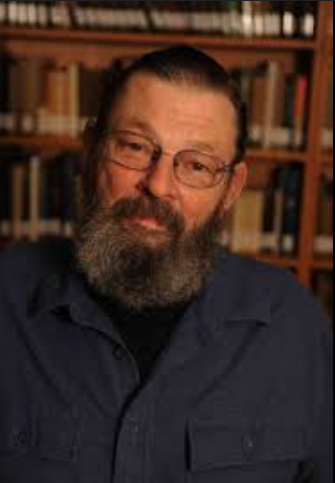
\includegraphics[width=0.6\linewidth]{imagens//secao1/haugeland1985.png}
            \caption{Prof. John Haugeland}
        \end{figure}
    \end{minipage}
    \begin{minipage}{0.5\linewidth}
        \begin{itemize}
        \justifying
            \item \textit{Artificial Intelligence: The Very Idea (1985).}
            \item \aspas{O novo e interessante esforço para fazer os
        computadores pensarem (...) máquinas com mentes, no
        sentido total e literal.}
        \end{itemize}
    \end{minipage}
\end{frame}

% Richard Bellman
\begin{frame}{O que é IA?}
    \begin{minipage}{0.5\linewidth}
        \begin{itemize}
        \justifying
            \item \textit{Artificial Intelligence (1972).}
            \item 
            \aspas{[Automatização de] atividades que associamos ao pensamento humano, atividades como a tomada de decisões, a resolução de problemas, o aprendizado...}
        \end{itemize}
    \end{minipage}
    \begin{minipage}{0.5\linewidth}
        \begin{figure}
            \centering
            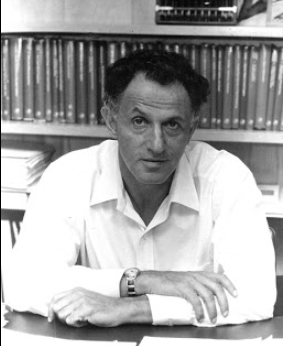
\includegraphics[width=0.6\linewidth]{imagens//secao1/bellman1978.png}
            \caption{Richard Bellman}
            \label{fig:enter-label}
        \end{figure}
    \end{minipage}
\end{frame}

% Raymond Kurzweil
\begin{frame}{O que é IA?}
    \begin{minipage}{0.5\linewidth}
        \begin{figure}
            \centering
            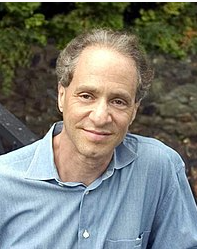
\includegraphics[width=0.5\linewidth]{imagens//secao1/kurzweil.png}
            \caption{Raymond Kurzweil}
        \end{figure}
    \end{minipage}
    \begin{minipage}{0.5\linewidth}
        \begin{itemize}
        \justifying
            \item \textit{The Age of Intelligent Machines (1990).}
            \item 
            \aspas{A arte de criar máquinas que executam funções que exigem inteligência quando executadas por pessoas.”}
        \end{itemize}
    \end{minipage}
\end{frame}

\begin{frame}{O que é IA? }
    \begin{itemize}
        \item 
        \aspas{
        O estudo das faculdades mentais pelo uso de modelos computacionais.
        }
        (Charniak e McDermott, 1985) 
        
        \item 
        \aspas{
        O estudo das computações que tornam possívelperceber, raciocinar e agir.
        }
        (Winston, 1992)
        
        \item 
        \aspas{
        O estudo de como os computadores podem fazer tarefas que hoje são melhor desempenhadas pelas pessoas.
        }
        (Rich and Knight, 1991)
        
        \item 
        \aspas{
        “Inteligência Computacional é o estudo do projeto de agentes inteligentes.
        }
        (Poole et al., 1998) 

        \item 
        \aspas{
        AI... está relacionada a um desempenho inteligente de artefatos.
        }
        (Nilsson, 1998)
    \end{itemize}
\end{frame}